\section{Introduction}

In recent years, indoor scene understanding has attracted wide attention due to its promising applications, including augmented/virtual reality and robotics. Massive researches have been carried out in related fields, such as semantic segmentation, room layout estimation and object detection. However, most of the previous work focused on solving the above problems with 2D images from a single perspective. The scenario information from a single view is quite limited and difficult to meet the requirements of practical high-level applications. In this paper, we try to explore the whole layout of an indoor scene using multi-view images.

Room layout estimation is a fundamental task within scene understanding. It aims to predict semantic boundaries among walls, ceiling and floor. Due to the development of deep neural networks, recent methods built on FCN have achieved remarkable performance in single-view images \cite{PIO,CFILE,DELAY,ICIP2018}. To make full use of contextual information for better understanding of an indoor scene, \cite{panocontext} present a whole-room 3D context model which take a \ang{360} panorama as input and then output the detected objects and room layout in 3D. They extends the techniques used in single-view images by projecting the panorama into multiple overlapping perspective images first. In a subsequent technique \cite{LayoutNet}, Zou et al. propose the LayoutNet network which trained directly on the panoramic image to estimate the 3D room layout. They achieve better performance in both accuracy and speed. However, it's not always convenient to obtain high-quality \ang{360} panoramic images in practical application. For this reason, we propose to explore the whole room structure using multi-view images as an alternative scheme.


By representing the entire room with multi-view images, we can naturally benefit from the mature techniques on perspective images. The estimated room layouts from different views can supplement each other and further improve the prediction accuracy of each perspective. Then we merge the prediction from multiple overlapping images and produce the holistic estimation of layout. The 3D structure of the entire room can be reconstructed from our holistic prediction, as depicted in Fig. \ref{fig:renderingResults}.

(add intro for multi-view layout estimation, there are two related papers using SFM) 

\section{Approach}
Given multiple images of an indoor scene from different views, our framework produces the corresponding whole-room layout estimation. Fig. \ref{fig:overview} shows the system overview. We first estimate the room layout seperately in multiple perspective images, details can be found in Sec. \ref{sec:layout}. Then the estimated room layouts are integrated into a panorama through image stitching. We average the prediction from different views to improve the overall accuracy, as described in Sec. \ref{sec:merging}. We further align the panorama to be level with the floor and reconstruct 3D structure of the room, as described in Sec. \ref{sec:align}. 

\begin{figure*}
	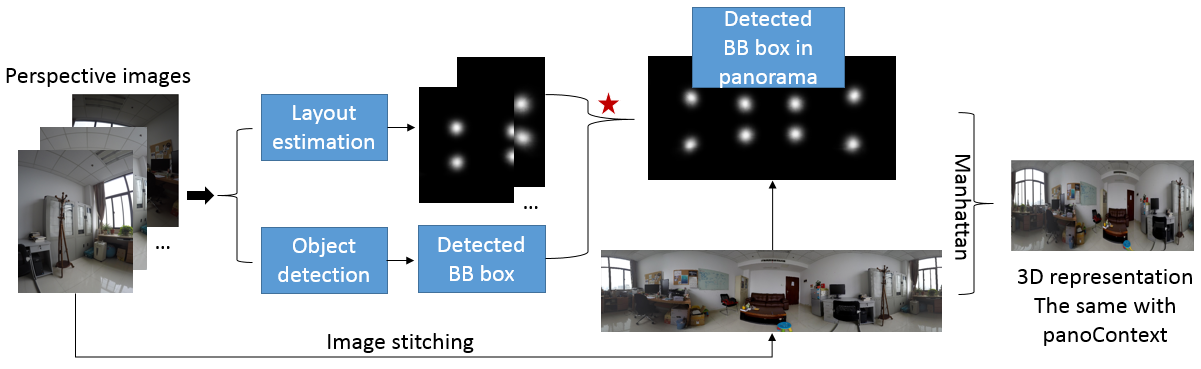
\includegraphics[height=2in, width=6in]{figs/ppline.png}
	\label{fig:overview}
	\caption{System overview.}
\end{figure*}

\subsection{Room Layout Estimation}
\label{sec:layout}
In this section, We are going to recover the room layout for perspective images from different views. Previous techniques of room layout estimation on perspective images typically represent the room layout as a segmentation of semantic surfaces including walls, ceilings and floors \cite{Delay,ours} or as the semantic boundaries or intersection points among them \cite{CFILE}. A direct way to achieve our goal is to utilize the existing methods to estimate the layout for each perspective, and then combine these representations to produce the whole-room 3D layout. However, this method is not efficient due to many redundant predictions caused by overlaps across views. To avoid redundant predictions or even to benefit from them, we propose a secondary representation of a room layout on perspective images. The room layout under each view is only represented by the intersections of two walls and ceiling or floor. We call these intersections secondary keypoints. Obviously, without the extra intersections of two semantic planes on the image boundaries, we cannot recover the room layout from a single perspective. However, these secondary keypoints in overlapping views are sufficient to reconstruct the 3D layout of the entire room. Compared to previous representations, our secondary keypoints are quite simplified and easier to train. It also naturally avoids a lot of redundant predictions. 
 
%We use an encoder-decoder Network structure proposed in \cite{RoomNet} to estimate room layouts on perspective images. The room layout is represented by a series of keypoints in a particular order. The keypoints are the intersection of different semantic planes on the the perspective images. By learning the location of these keypoints, a room layout can be reconstructed by simply connect these keypoints in a specific order.

\noindent\textbf{Network Architecture.} We adopt the encoder-decoder architecture proposed by \cite{roomnet} with modifications. The encoder part consists of 13 convolutional layers, which are topologically identical to the VGG16 network. It encodes the $320\times320$ input images to $10\times10$ feature maps. Then we modify the decoder part to upsample the feature maps from the bottleneck layer with low resolution to full input resolution. As our simplified representation no longer depends on the topological category of the room, we further remove the classification branch. 

\begin{figure}
	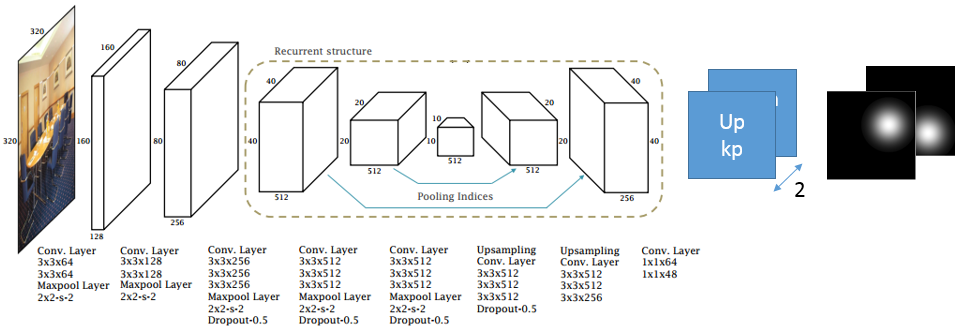
\includegraphics[height=1.5in, width=3in]{figs/network.png}
	\label{fig:network}
	\caption{Network architecture.}
\end{figure}

\noindent\textbf{Training.} The secondary keypoints can be divided into two categories according to semantics: the intersection of two walls and ceiling or the intersection of two walls and floor. We train the network to regress these two kinds of keypoints seperately in order to eliminate the ambiguity between them. For this reason, the output of our network is a $w \times h \times 2$ probability array $T$, where $w$ and $h$ stand for the width and length of the input image. Each of the 2 slices can be viewed as a probability map for the secondary keypoints in a corresponding category. We adopt the PanoContext dataset \cite{pano} and relabeled Stanford 2D-3D dataset \cite{layoutnet} to train our layout estimation network. To obtain multiple overlapping perspective images, we project the panoramic images into different views using the toolkit provided by \cite{pano}. The ground truth of the secondary keypoints is represented by several 2D Gaussian heatmaps centered at their locations. We adjust the distribution imbalance between foreground and background pixels by degrading the gradient weight of background pixels with a coefficient of 0.2.

%The RoomNet-basic struture in \cite{RoomNet} is adopted in our training stage for efficiency. We first pretrain the Network on LSUN \cite{LSUN2016} training set. Then, to finetune the model on images from different views in the same room, we project the panorama from \cite{PanoContext} to $k$ views. We set $k$ to 12 and 24 in our experiment. The layout ground truth is relabeled using the same projection. 


\subsection{Generation of Panorama}
\label{sec:merging}
In this section, we combine the predicted layouts from different perspectives and generate a panoramic layout estimation. Fisrt, we stitch the input multi-view images into a panoramic image. Then, we use the same mapping to map the predicted probability array $T$ from different views into a panoramic predictions and averaged across views. To reduce the noise caused by false predictions from specific perspectives, we calculate the LOG response of the panoramic predictions at a certain scale (depending on the radius of the keypoints), $\sigma$ is set to 21 in our case. After that, we sum up the probability maps from two channel to get a holistc probability map. Finally, we follow the post-processing method in \cite{LayoutNet} to obtain the locations of the keypoints in the panorama. In brief, the holistic probability map are summed across rows to find four local maxima for columns, then two largest peaks are found along each of the four columns. In this way, we attain the location of eight keypoints for each panorama. Then the whole room layout can be reconstructed by connecting these eight keypoints.


\subsection{Alignment and 3D Reconstruction}
\label{sec:align}

(Optional and undone) In this section, we align the panoramic images to make sure that wall-wall boundaries are vertical to the floor. If we use the panorama to generate testing images, this step can be omitted as the reprojected panoramic images naturally met this alignment condition. Then the aligned panorama can be further rendered into a 3D representation. These two steps are implemented using existing techniques but the rendering part is not yet available. 


\section{Results}
Experiments, three parts: one for different field of view (FOV), one for comparison with panorama based method, the last one for qualitative results.

\begin{table}
	\caption{Results of different FOV.}
	\label{tab:FOV}
	\begin{tabular}{cccc}
		\toprule
		FOV &3D IoU (\%)&Corner error (\%)&Pixel error (\%)\\
		\midrule
		 60 & XX & XX & XX\\
		90 & XX & XX & XX\\	
		\bottomrule
	\end{tabular}
\end{table}

\begin{table}
	\caption{Quantitative results on PanoContext dataset.}
	\label{tab:PC}
	\begin{tabular}{cccc}
		\toprule
		Method&3D IoU (\%)&Corner error (\%)&Pixel error (\%)\\
		\midrule
		PanoContext & 67.23 & 1.60 & 4.55\\
		LayoutNet & 74.48 & 1.06 & 3.34\\
		Our Method & 59.58 & 2.20 & 6.78\\		
		\bottomrule
	\end{tabular}
\end{table}

\section{Conclusions}
In this paper, we propose a method to estimate the overall room layout based on multiple views. 


\begin{acks}
  The authors would like to thank ...
\end{acks}
